\documentclass[conference,compsoc]{IEEEtran}
% *** MISC UTILITY PACKAGES ***
%
\usepackage{url}
% *** CITATION PACKAGES ***
%
\ifCLASSOPTIONcompsoc
  % IEEE Computer Society needs nocompress option
  % requires cite.sty v4.0 or later (November 2003)
  \usepackage[nocompress]{cite}
\else
  % normal IEEE
  \usepackage{cite}
\fi

% *** GRAPHICS RELATED PACKAGES ***
%
\ifCLASSINFOpdf
  \usepackage[pdftex]{graphicx}
\else
  \usepackage[dvips]{graphicx}
\fi
% *** MATH PACKAGES ***
%
\usepackage{amsmath}
% *** SUBFIGURE PACKAGES ***
\ifCLASSOPTIONcompsoc
  \usepackage[caption=false,font=footnotesize,labelfont=sf,textfont=sf]{subfig}
\else
  \usepackage[caption=false,font=footnotesize]{subfig}
\fi

\hyphenation{bet-ween}


\begin{document}

\title{Topic mining for short-text documents on micro-blogging site\\ by combining Doc2Vec and clustering techniques}


% author names and affiliations
% use a multiple column layout for up to three different
% affiliations
\author{\IEEEauthorblockN{Thuong-Hai Pham}
\IEEEauthorblockA{Faculty of Information and Communication Technology\\
University of Malta\\
Msida MSD 2080, Malta\\
Email: thuong-hai.pham.16@um.edu.mt}
}

% make the title area
\maketitle

% As a general rule, do not put math, special symbols or citations
% in the abstract
\begin{abstract}
In the era of data explosion these days, especially digital text generated by World-Wide-Web users, it demands techniques that automatically organize large collection of text for further analysing and processing tasks. One family of those techniques is called ``topic model". These techniques discover underlying topics from a given corpus with or without intervention of human, in other word, supervised and unsupervised. This report is aimed to examine the traditional Latent Dirichlet Allocation (LDA) and a proposed method of combining Doc2Vec and clustering technique on the problem of topic mining. For practical evaluation, Twitter\footnote{https://twitter.com/} is chosen to do experiment on three approaches: standard LDA, author-topic model and our proposed approach. The paper also covers background behind each method and proposes a plan to conduct this research on these approaches with estimated time-line and resources.
\end{abstract}

% no keywords

\section{Introduction}

Applying topic model for micro-blogging site is a very important task to enhance our understanding of the social network. One very successful technique and also being considered as state-of-the-art in unsupervised topic model is Latent Dirichlet Allocation (LDA)\cite{Blei2003}. Some applications were proposed by Zhao et al. (2011) \cite{zhao2011comparing} with the work of comparing Twitter and traditional media by LDA, or finding topic-sensitive influencers on Twitter by Weng et al. (2010) \cite{Weng2010}.

It is important to be noted that applying LDA directly on micro-blogging sites is considered to be not a trivial task yet more challenging problem. This occurs due to the nature of micro-blogging sites which is the limited length of each posting unit (e.g. tweets on Twitter have maximum 140 characters each). In addition, proposed LDA solution while trying to solve this problem have to make more assumptions (single-topic tweets...)\cite{zhao2011comparing} about the data itself rather than the bag-of-words (BoW) assumption from original LDA.

Therefore, we consider examining clustering method such as K-means to discover the underlying topic. The feature learning is done by doc2vec of Le \& Mikolov\cite{le2014distributed}, which is an adaptation of word2vec\cite{mikolov2013distributed}.


For the rest of this paper, in section \ref{background}, we discuss about the mathematical background behind BoW assumption for topic model: the infinite exchangeability and De Finetti theorem. Thereafter, we revise LDA as a generative probabilistic model and its latent variables in section \ref{lda}. However, LDA does not work well when applying directly to short-text documents as tweets, we then consider two variants of LDA to solve this problem which are author-topic model (\ref{author_topic}) and Twitter-LDA (\ref{twitter_lda}). To end with the background and related works, the three groups of methods to evaluate topic models are also mentioned in section \ref{evaluation}. To the most important part, we figure out the disadvantages of these methods and present our proposal (section \ref{proposal}). Also in this section, we breakdown the required tasks, its timeline, and needed resources with expected result and challenges we may face.


\section{Background} \label{background}


\subsection{Mathematical background} \label{math}

\subsubsection{Exchangeability}

We say that $(x_1,x_2...)$ is an infinitely exchangeable sequence of random variables if, for any $n$, the joint probability $p(x_1,x_2,...,x_n)$ is invariant to permutation of the indices. That is, for any permutation $\pi$,
\[p(x_1,...,x_n) = p(x_\pi(1),...,x_\pi(n))\]
It is important to emphasize that independent and identically distributed random variables are always infinitely exchangeable. However, infinite exchangeability is a much broader concept than being independent and identically distributed. 
%For example, let $(x_1,x_2,\dots)$ be independent and identically distributed, and let $x_0$ be a non-trivial random variable independent of the rest. Then $(x_0+x_1,x_0+x_2,\dots)$ is infinitely exchangeable but not independent and identically distributed.

\subsubsection{De Finetti theorem, 1935}
A sequence of random variables $(x_1,x_2,...)$ is infinitely exchangeable iff,for all $n$,
\[p(x_1,x_2,...,x_n)=\int\prod_{i=1}^{n}p(x_i|\theta)P(d\theta)\]
for some measure $P$ on $\theta$.
If one assumes the data is infinitely exchangeable, then there must exist an underlying parameter and prior.

\subsection{Latent Dirichlet Allocation} \label{lda}

LDA is a generative probabilistic model of a corpus. The basic idea is that documents are represented as random mixtures over latent topics, where a topic is characterized by a distribution over words. To implement this idea, LDA assumes each document is a bag of words (BoW assumption). Hence, it applies infinite exchangeability on the documents and inherits the De Finetti theorem to expect an latent parameter and prior underlying in the corpus. These latent variables are illustrated in the figure \ref{fig:lda_model} below.


\begin{figure}[h]
	\centering
	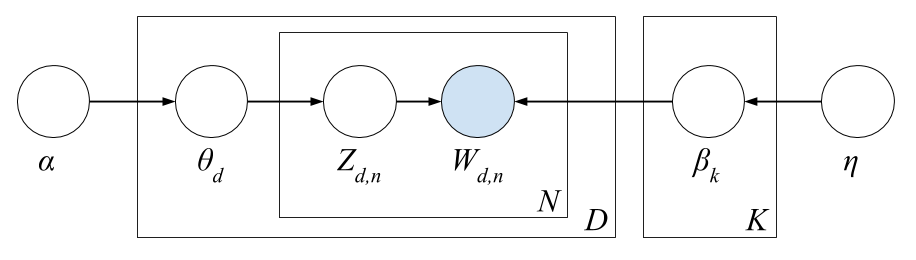
\includegraphics[scale=0.2]{lda_model}
	\caption{LDA graphical model}
	\label{fig:lda_model}
\end{figure}

In figure \ref{fig:lda_model}:
\begin{itemize}
	\item $\alpha$ is Dirichlet distribution parameter, controls the shape and sparsity of $\theta$
	\item $\theta$ are per-document topic proportions.\\
	$\theta$ is a K-dimensional Dirichlet random variable, takes values in the (k-1)-simplex, and has the following probabiltiy density on this simplex:
	\[p(\theta|\alpha)=\frac{\Gamma(\sum_{i=1}^{K}\alpha_i)}{\prod_{i=1}^{K}\Gamma(\alpha_i)}\theta_1^{\alpha_1-1}\dots\theta_K^{\alpha_K-1}\]
	The Dirichlet is conjugate to the multinomial. Given a multinomial observation, the posterior distribution of $\theta$ is a Dirichlet.
	\item $Z_{d,n}$ is per-word topic assignment, in which $D$ and $N$ are number of documents and number of words in a specific document, respectively.
	\item $W_{d,n}$ is observed word.
	\item $\beta$ are topics, which is $V$ dimensional Dirichlet.
	\item $\eta$ is the topic hyper parameter.
\end{itemize}

The blue-shaded node denotes observed variable, the others are hidden or latent variables. Plates denote replicated structures.

From a collection of documents, LDA infers: per-word topic assignment $Z_{d,n}$, per-document topic proportions $\theta_d$ and per-corpus topic distributions $\beta_k$.

%\subsubsection{Generative process}
%
%As mentioned above, LDA is a generative probabilistic model, which generative process is performed as described below:
%\begin{enumerate}
%	\item Draw $\theta_d \sim Dir(\alpha)$
%	\item Draw $\beta_k \sim Dir(\eta)$
%	\item For each of the N words in document d $W_{d,n}$:
%	\begin{enumerate}
%		\item Draw a topic $Z_{d,n} \sim Multinomial(\theta_d)$
%		\item Draw a word $W_{d,n}$ from $p(W_{d,n}|Z_{d,n},\beta)$, a multinomial probability conditioned on the topic $Z_{d,n}$
%	\end{enumerate}
%\end{enumerate}
%
%\subsubsection{Model inference}
%However, in the real problem, to acquire underlying latent topics, we have to reverse the generative process by solving an inferential problem. The main goal of this inferential problem is to compute the posterior distribution of the latent variables in figure \ref{fig:lda_model}:
%\[p(\theta,Z|W,\alpha,\beta)=\frac{p(\theta,Z,W|\alpha,\beta)}{p(W|\alpha,\beta)}\]
%
%The function $p(\theta,Z|W,\alpha,\beta)$, in practice, is not possible to compute. Due to the conjugacy of Dirichlet distribution, we can marginalize over latent variables to rewrite the posterior $p(W|\alpha,\beta)$. This posterior is still hardly be inferred exactly. Nevertheless, there exist a wide variety of approximate inference algorithms for LDA:
%\begin{itemize}
%	\item Mean field variational methods \cite{blei2004variational} (Blei et al., 2001)
%	\item Expectation propagation \cite{minka2002expectation} (Minka and Lafferty, 2002)
%	\item Collapsed Gibbs sampling \cite{griffiths2004finding} (Griffiths and Steyvers, 2004)
%	\item Collapsed variational inference \cite{teh2006collapsed} (Teh et al., 2006)
%\end{itemize}
%
%After being approximated, beside LDA, the posterior can be used in many other applications such as collaborative filtering, document similarity and information retrieval...

\subsection{Latent Dirichlet Allocation variants for Twitter} \label{lda_app}

One very basic approach is to apply LDA directly to Twitter by treating each tweet as a single document. However, due to the constraint of 140 characters per tweet, a tweet is too short for LDA to figure out the topic proportions.

\subsubsection{The author-topic model} \label{author_topic}

To overcome this issue, by excluding the topic proportions for each tweets but taking into consideration only the underlying topics in each user, aggregating all tweets of a Twitter's user into a single document was proposed and gained a better result to direct LDA \cite{Weng2010,hong2010empirical}.

On one hand, this approach is very efficient on a specific task (e.g. topic-sensitive influencers mining \cite{Weng2010}) by not modifying the inference process of original LDA. On the other hand, the target of this approach is each user, not tweets, so it is not applicable for a general problem of topic mining.

\subsubsection{Twitter-LDA} \label{twitter_lda}

On a different perspective, while attempting to compare Twitter and traditional media, Zhao et al. \cite{zhao2011comparing} proposed Twitter-LDA, a modified version of LDA to work on Twitter's short tweets without concatenating all tweets into one.

\begin{figure}[h]
	\centering
	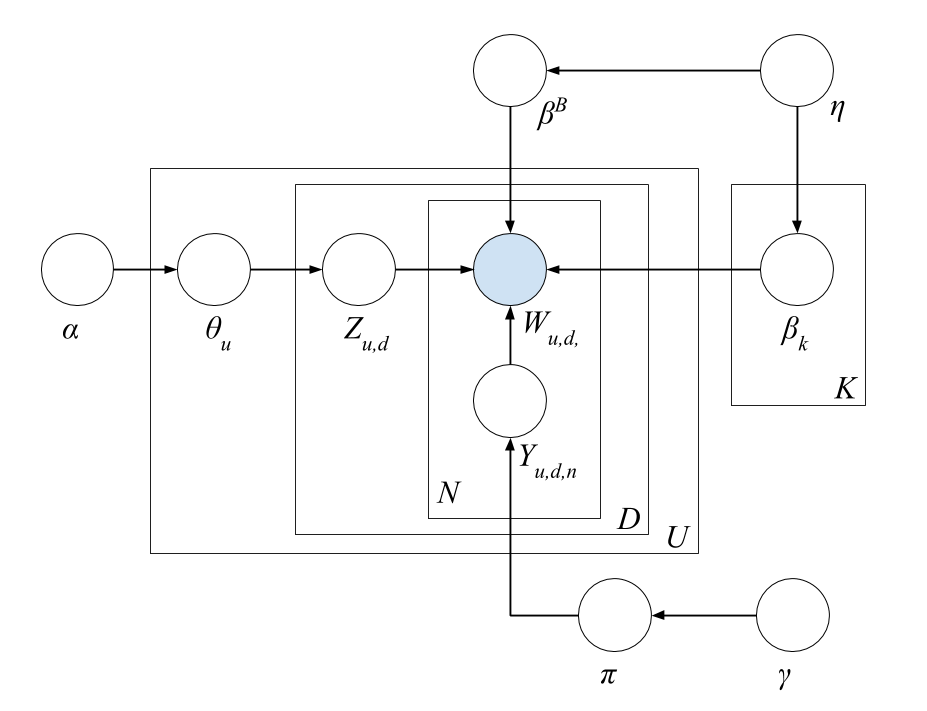
\includegraphics[scale=0.2]{twitter_lda_model}
	\caption{Twitter-LDA graphical model}
	\label{fig:twitter_lda_model}
\end{figure}

In figure \ref{fig:twitter_lda_model}, the author introduced four more variables:
\begin{itemize}
	\item $\beta^B$ denotes the background words distribution
	\item $\pi$ denotes a Bernoulli distribution which simulate the choice of authors between topic-related words and background words.
	\item $\gamma$ is the parameter of distribution $\pi$.
	\item $Y_{u,d,v}$ denotes the selection of background or topic word.
\end{itemize} 
and a slightly modification on $\theta$ that $\theta_u$ represents per-user topic proportions instead of per-document as in the original version. In addition, the D (document) plate is surrounded by a new plate U which stands for each user. It is necessary to mention that Twitter-LDA makes an assumption in which each tweet only conveys a single topic. We will clarify our disagreement on this assumption in section \ref{proposal}.

%By defining the model as in figure \ref{fig:twitter_lda_model}, the generative process of Twitter-LDA is performed as followed:
%\begin{enumerate}
%	\item Draw $\beta^B \sim Dir(\eta)$
%	\item Draw $\pi \sim Dir(\gamma)$
%	\item Draw $\beta_k \sim Dir(\eta)$
%	\item For each user,
%	\begin{enumerate}
%		\item Draw $Z_{u,d} \sim Multi(\theta_u)$
%		\item For each word in document d,
%		\begin{enumerate}
%			\item Draw $Y_{u,d,n} \sim Multi(\pi)$
%			\item Draw \[W_{u,d,n} \sim 
%			\begin{cases}
%			Multi(\theta^B) & \text{if $Y_{u,d,n} = 0$}\\
%			Multi(\theta^{Z_{u,d}}) & \text{if $Y_{u,d,n} = 1$}
%			\end{cases}\]
%		\end{enumerate}
%	\end{enumerate}
%\end{enumerate}

\subsection{Evaluation} \label{evaluation}

Wallach et al. \cite{Wallach2009a} summarized a variety of methods to evaluate LDA. As a topic model method, LDA is commonly evaluated by intrinsic and extrinsic evaluation. 

\subsubsection{Intrinsic evaluation}
One very basic intrinsic evaluation method is to view the problem as document modelling \cite{Blei2003}. By stating that, the goal of the model is to achieve high likelihood on a held-out test set, $C'$. In this case, the perplexity measure is used as in normal language modelling problem, in which the lower perplexity, the better performance the model achieves.
\[perp(C')=exp\left\{-\frac{\sum_{d=1}^{D}{log(p(W_d))}}{\sum_{d=1}^{D}N_d}\right\}\]

More advanced, measurement is also estimated by the probability of unseen held-out documents given some training documents. This probability can be written as \cite{Wallach2009a}
\[P(C|C')=\int d\theta d\alpha dm P(C|\theta,\alpha m)P(\theta,\alpha m|C').\]
in which, $C, C'$ denote training documents set (corpus) and held-out documents set, respectively. Noted that $m$ is the base measure of Dirichlet distribution, in addition to the concentration parameter $\alpha$.

%There is also a variation of this method, document completion, which compare predictive performance by estimating the probability of the second half of each document given the first half. In this point of view, let $c^{(1)}$ be the first half and $c^{(2)}$ be the second half, the goal of our measurement is to compute
%\[P(w^{(2)}|w^{(1)},\theta,\alpha m)=\frac{P(w^{(2)}, w^{(1)}|\theta,\alpha m)}{P(w^{(1)}|\theta,\alpha m)}\]

\subsubsection{Extrinsic evaluation}
On the other hand, extrinsic approaches measure LDA performance on some secondary tasks, such as corpus comparison \cite{zhao2011comparing} or topic-sensitive influencers mining \cite{Weng2010}. These approaches are similar to the way language models performance are measured.

\subsubsection{Human evaluation}

As a part of the corpus comparing work \cite{zhao2011comparing}, Zhao et al. also evaluated the performance between original LDA, author-topic model and their proposed Twitter-LDA. Based on preliminary experiments, the authors set number of topic K to 110 for each model, then mixed 330 topics from the three models. The topics were then scored by two human judges. Each assigned a score on each topic, ranging from 1 (meaningful) to 0 (nonsense).

% The result showed that Twitter-LDA gained 25.23\% higher in term of average score to author-topic model, and 32.61\% higher then standard LDA. Hence, Twitter-LDA obviously outperformed the two previous methods and were used in their comparison task.


\section{Proposed method} \label{proposal}

The two methods of author-topic model and Twitter-LDA have overcome the problem of short tweets in the micro-blogging site Twitter which prevent direct usage of original LDA. More than that, Twitter-LDA has showed to outperform the other two in experiment. Nevertheless, Twitter-LDA has to change the original LDA process and inference approximation algorithm to implement its idea. This approach is hard to be re-implemented in industrial sector by using existed library for other problems.

More than that, it is worth to consider the assumption of one tweet belongs only to one topic. One topic may represents only one topic intended by its Twitter user. However, please note that this topic is not the final topic discovered by our mining methods but may be a combination of the two final topics. For example, the topic user intend to tweet about is public insurance. Throughout the whole corpus, our mining process points out two distinct topics: healthcare and public administration. It is obvious that the user-intended topic reflects both of our discovered topics on the perspective of the whole corpus.

Bearing that in mind, we would like to propose a method to compare with original LDA and author-topic model, by accepting only BoW assumption.

\subsection{Clustering based on distributed representation of sentences} \label{doc2vec}

\subsubsection{Distributed representation of sentences for features learning}
After word2vec\cite{mikolov2013distributed}, Le and Mikolov presented the paragraph (document) vector models. Formally, the objective of a word embedding model  is to maximise the log probability
\[\frac{1}{T}\sum_{t=k}^{T-k}\log p(w_t|w_{t-k},\dots,w_{t+k}) \]
given a sequence of training words $w_1,w_2,w_3,\dots,w_T$.

The paragraph vector models uses the same idea to develop the paragraph vector framework. In fact, this is not a single model but implemented into two different approaches: Distributed Memory model (DM) and Distributed Bag of Words (DBOW) - vector without word ordering.

\begin{figure}[h]
	\centering
	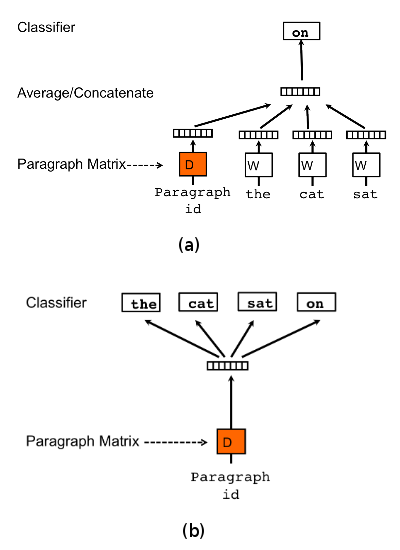
\includegraphics[scale=0.5]{doc2vec}
	\caption{Framework for learning paragraph vector, (a) Distributed Memory, (b) Distributed Bag of Words}
	\label{fig:doc2vec}
\end{figure}

In figure \ref{fig:doc2vec} above\footnote{https://arxiv.org/pdf/1405.4053v2.pdf}, the DM model (a) is actually constructed from each word vector of that structure (sentence/document), then these vectors are combined (through averaging or concatenation) to learn the sentence/document features. In addition, a paragraph matrix is maintained to keep track of the whole sentence/document. In contrary to that, the DBOW model does not combine any word vectors yet only a paragraph vector is trained to predict the context.

\begin{figure*}[tb]
	\centering
	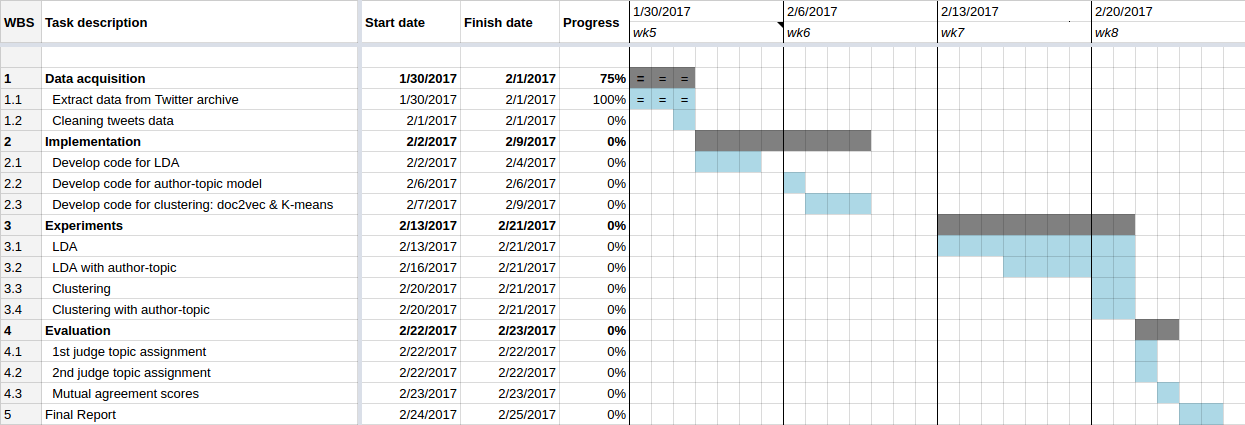
\includegraphics[width=\textwidth]{project_timeline}
	\caption{Project timeline}
	\label{fig:project_timeline}
\end{figure*}

\subsubsection{Clustering based on the learned features}
Our proposed method consists of two distinguished phases. First, ``meaning" or, in fact, features of each document is learned by doc2vec model as presented above. Having the features, the documents are then clustered using clustering technique. 

For the goal of our experiment described latter in \ref{evaluation}, we choose K-means to find hard clusters from our documents, each cluster represents a topic. However, to produce a probabilistic topic proportions as in LDA, we can easily change K-means to C-mean to achieve fuzzy or soft clusters.

\subsection{Tasks} \label{tasks}

The project is planned into four main phases: data acquisition, implementation, experiments and evaluation phase. Figure \ref{fig:project_timeline} illustrates sub-tasks in each phases and their estimated required working time.


To be more detailed, data for this project is acquired from Twitter stream archive\footnote{https://archive.org/details/archiveteam-twitter-stream-2016-07} in July 2016. Although we do not need to stream data directly from streaming API, data preprocessing still plays an essential role to filter out other languages (Chinese, Japanese, Spanish...) tweets, remove stop-words, tokenize words within tweets, remove urls and normalise unconventional language used on social media (character repetition, emoticons...)

Source-code used for the latter evaluation is developed using LDA and Doc2Vec model in Gensim\footnote{\url{https://radimrehurek.com/gensim/}} library.

For the evaluation task, although perplexity is considered to justify the result with less subjectivity, it does not measure how meaningful the topics discovered. Hence, we make use of the human evaluation strategy\cite{zhao2011comparing} instead. This evaluation process is performed by two distinct judges. Each judge assigns name for all of the topics in our output results. Afterwards, their topic name assignments are exchanged to each other to score from 0 to 10 how they agree with the other judge about the topic names. The meaningfulness of each algorithm and parameter pair is measured by averaging all the agreement score above, which basically reflect the interpretability of the result.

\subsection{Resources} \label{resources}

Due to the magnitude of our data (48.7GB in compressed format), a sufficiently efficient machine is required to perform data preprocessing and calculation for our experiment. Therefore, we intend to make use of the Google cloud compute engine n1-standard-4\footnote{operates with 4 virtual CPUs, 15GB RAM, 200GB hard disk drive}. In addition, the experiment evaluation process also required to employ 2 judges (the more, the better) to individually score meaningfulness of our topic mining result.

\section{Expected result \& difficulties} \label{expectation}

Our hypothesis for this is the proposed method of combining Doc2Vec and K-means achieves approximate meaningfulness score in compare to traditional LDA method. This expectation also implies that the proposed method can perform equally or better by having no assumption, which is subjective and arguably untrue, about the data itself.

On the other hand, we anticipate to face with some difficulty regards to data. Firstly, Twitter stream archive is too large and prevent us to consume all of the available tweets for our models. Hence, we have to prioritise tweets to be fed to our models by the number of tweets per user. Only top tweeted users are being taken into consideration. This strategy also support in making the difference when running author-topic model. Secondly, the acquired data may contains too much noise and unconventional language usage. Thirdly, the meaning of topic discovered can be unclear or hardly interpretable because of the fact that most tweets are about their daily life instead of broad topic coverage in newspaper. These two latter obstacles can be solved in some degree by careful cleaning of raw data in our data acquisition phases.

\bibliographystyle{IEEEtran}
\bibliography{summarize}


\end{document}
